\documentclass[12pt]{article} 
\usepackage{geometry} 
\geometry{a4paper} 
\linespread{1.1} % Line spacing


% FIGURES AND FLOATS
\usepackage{graphicx} % Required for including pictures
\usepackage{float} % Allows putting an [H] in \begin{figure} to specify the exact location of the figure
\usepackage{wrapfig} % Allows in-line images such as the example fish picture
\usepackage[font={small,it}]{caption}
\usepackage{subcaption}
\usepackage{epstopdf}
\graphicspath{{images/}}
\usepackage{diagbox}

% MATH
\usepackage{amssymb}
\usepackage{amsmath}
\usepackage{algorithm}
\usepackage[noend]{algpseudocode}

% OTHER
\usepackage[]{mcode}
\usepackage{enumerate}
\usepackage{xcolor}


%character
\usepackage{indentfirst} % 强制要求第一个段落也进行缩进
%段间距
\setlength{\parskip}{1ex plus 0.5ex minus 0.5ex}
%%%%%%%%%%%%%%%%%%%%%%%%%%%%%%%%%%%%%%%%%%%%%%%%%%%%%%%%%%%%
\usepackage{listings} 

%段首缩进
\setlength{\parindent}{2em} 

\definecolor{DeepPink}{RGB}{255, 20, 147}
\definecolor{LightSlateBlue}{RGB}{132, 112, 255}
\definecolor{ForestGreen}{RGB}{34, 139, 34}

\lstset{
  language=Matlab,  %代码语言使用的是matlab
  frame=shadowbox, %把代码用带有阴影的框圈起来
  rulesepcolor=\color{red!20!green!20!blue!20},%代码块边框为淡青色
  keywordstyle=\color{blue!90}\bfseries, %代码关键字的颜色为蓝色,粗体
  commentstyle=\color{ForestGreen}\textit,    % 设置代码注释的颜色
  showstringspaces=false,%不显示代码字符串中间的空格标记
  numbers=left, % 显示行号
  numberstyle=\tiny,    % 行号字体
  stringstyle=\ttfamily, % 代码字符串的特殊格式
  basicstyle={\small\ttfamily},
  breaklines=true, %对过长的代码自动换行
  extendedchars=false,  %解决代码跨页时,章节标题,页眉等汉字不显示的问题
  texcl=true,
  % basicstyle=\fontfamily{Microsoft YaHei}\selectfont\footnotesize, % 设置字体族为微软雅黑,字号为footnotesize
}

\lstset{breaklines}%自动将长的代码行换行排版

\lstset{extendedchars=false}%解决代码跨页时,章节标题,页眉等汉字不显示的问题
%%%%%%%%%%%%%%%%%%%%%%%%%%%%%%%%%%%%%%%%%%%%%%%%%%%%%%%%%%%%
\title{\LARGE Solution to analysis in Home Assignment 4 \\  \vspace{1cm}\Large }
\author{Yongzhao Chen(yongzhao@chalmers.se)}
\date{\vspace{8cm}\today}
\begin{document}
\maketitle
\thispagestyle{empty}
\newpage
%%%%%%%%%%%%%%%%%%%%%%%%%%%%%%%%%%%%%%%%%%%%%%%%%%%%%%%%%%%%
\section{Smoothing}
\subsection{Task a}

In this part, mainly use the code from HA3 Q3, but use \texttt{nonLinRTSsmoother} function to generate the filtered output and the smoothed output.

And I realized my last HA3 had some bug, after the fix, the tuning value is chosen as :

\begin{equation}
    \begin{aligned}
        sigma_v = 10;\\
sigma_w = pi/180*6;\nonumber
    \end{aligned}
\end{equation}

The result shown in figure \ref{taska}, legends are detailed. To be more readable and to concentrate on the differences, the picture is zoomed in:

\begin{figure}[H]
 \centering
 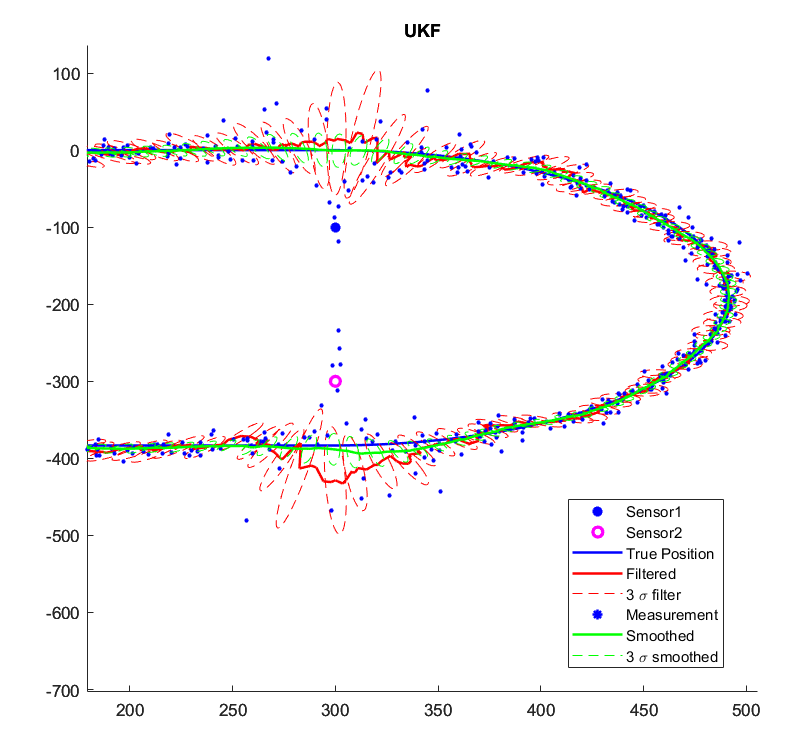
\includegraphics[width=0.7\textwidth]{images/taska.png}
 \caption{Task a: Comparison}
 \label{taska}
\end{figure}

\subsubsection{Conclusion}

From figure \ref{taska}, the green curve, which represents the smoothed output is closer to the true position line compare with the red curve, which represents the filtered output.

And from the $ 5_{th} $ curves, the covariances of the smoothed output are smaller than the filtered one.

\subsection{Task b}

I increased the value at $k=300$  by $ 10\% $ when generating true state $ X $ to see the result:

\begin{lstlisting}
    for i = 2:K+1
    if i ==300
    X(:,i) = 1.1*coordinatedTurnMotion(X(:,i-1),T);
    X(5,i) = 1.1*omega(i);
    else
    X(:,i) = coordinatedTurnMotion(X(:,i-1),T);
    X(5,i) = omega(i);
    end
end
\end{lstlisting}

\begin{figure}[H]
 \centering
 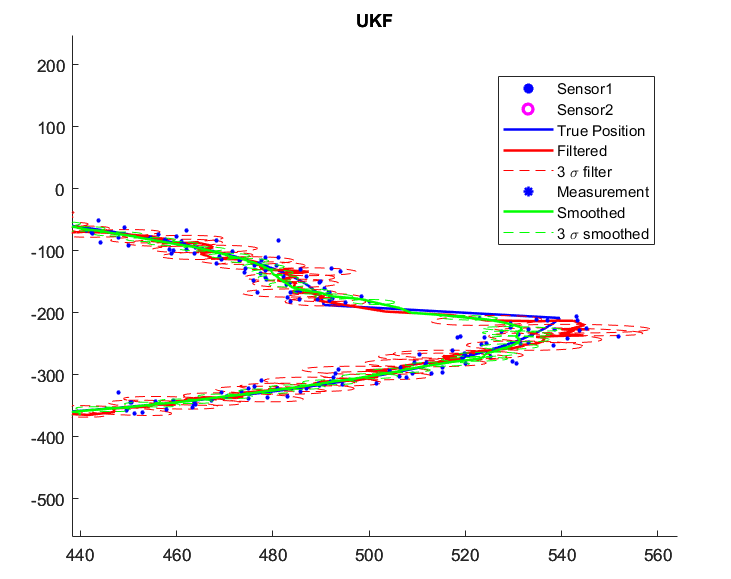
\includegraphics[width=0.7\textwidth]{images/taskb.png}
 \caption{Task b: Manually outlier}
 \label{Taskb}
\end{figure}

From figure \ref{Taskb}, the filtered output of the red curve follows the change of my manual outlier value, and has a big covariance at that point, while the smoothed output of the green curve goes less to the wrong value and has a smaller covariance compare to the filtered curve.

In summary, the filter is trying to incorporate the most recent measurement, including the outlier, into its estimate, while the smoother takes into account both past and future measurements when updating its estimate. As a result, the smoother can mitigate the effect of the outlier by considering the overall trajectory of the object and recognizing that the outlier is inconsistent with the other measurements.
\section{Task 2}

In this task, I placed the phone on the table without any touch or movement. 

When the phone is placed flat on a table, the accelerometer should read the gravitational acceleration on the Z-axis, while the readings on the X and Y axes should be zero.
The readings of the gyroscope should be zero in all three directions, while the magnetometer readings should reflect the magnetic field strength of the phone's current position.

Since the last moment I touched the screen to stop stream, so in calculation I throwed the last 0.1 second data away to avoid disturbances.

\subsection{True state}

\begin{figure}[H]
 \centering
 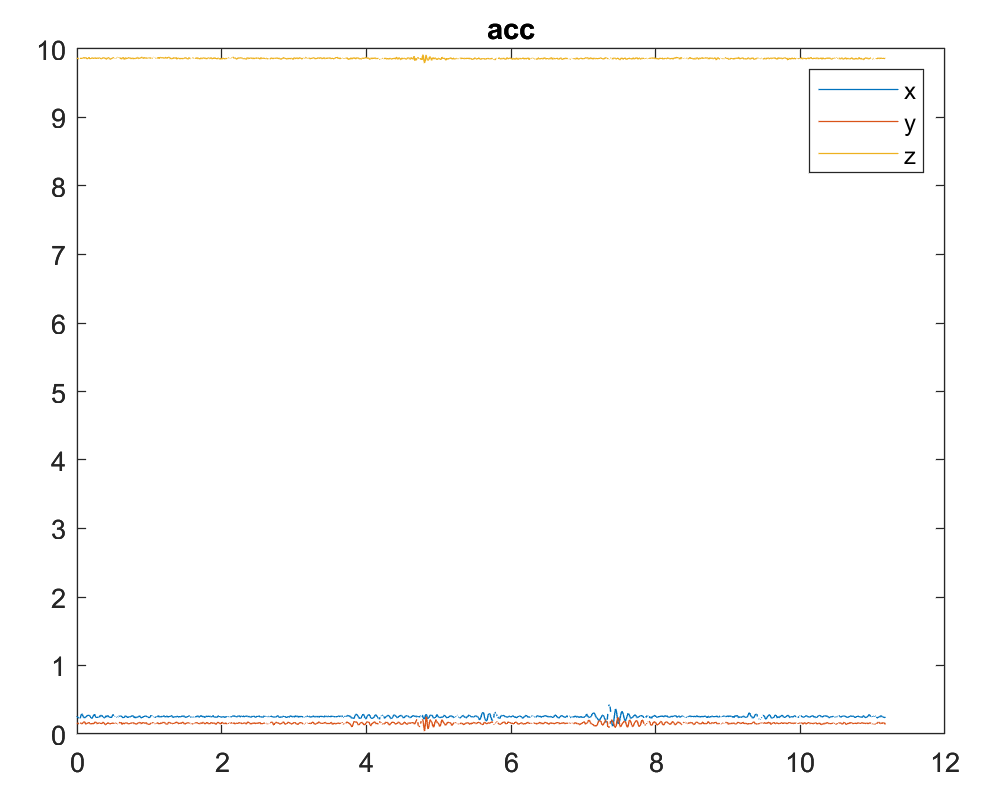
\includegraphics[width=0.7\textwidth]{images/acc.png}
 \caption{Accelerometers}
 \label{acc}
\end{figure}

\begin{figure}[H]
 \centering
 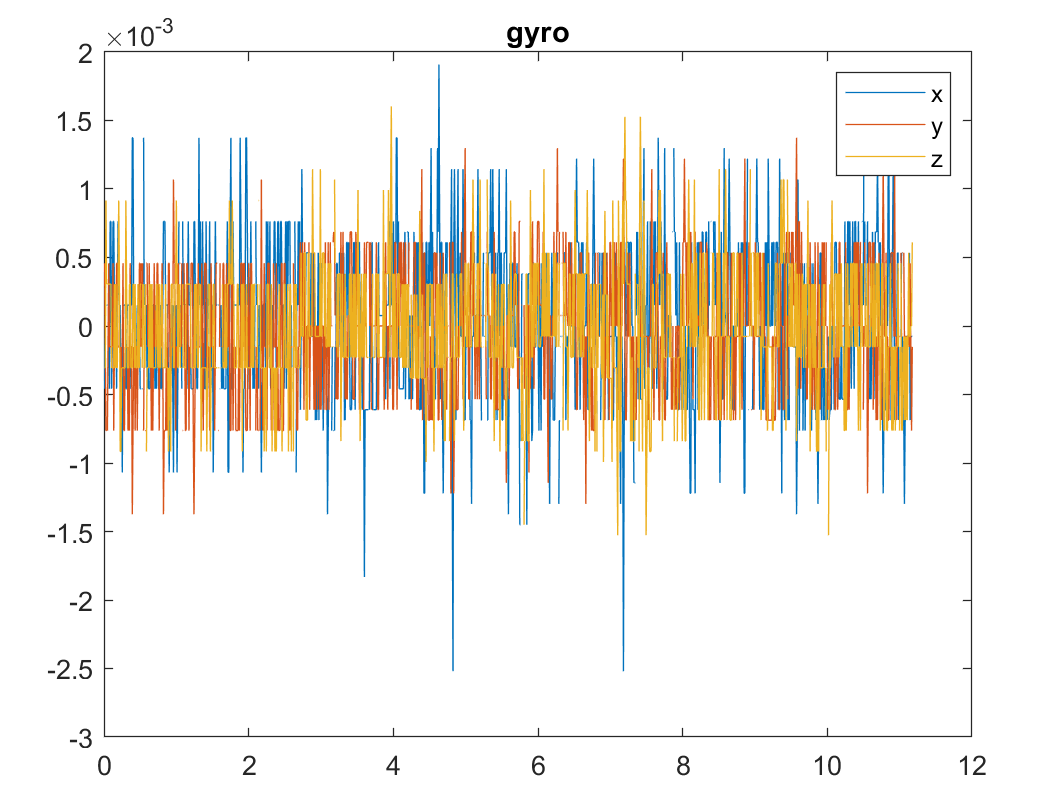
\includegraphics[width=0.7\textwidth]{images/gyroscope.png}
 \caption{Gyroscope}
 \label{gyro}
\end{figure}

\begin{figure}[H]
 \centering
 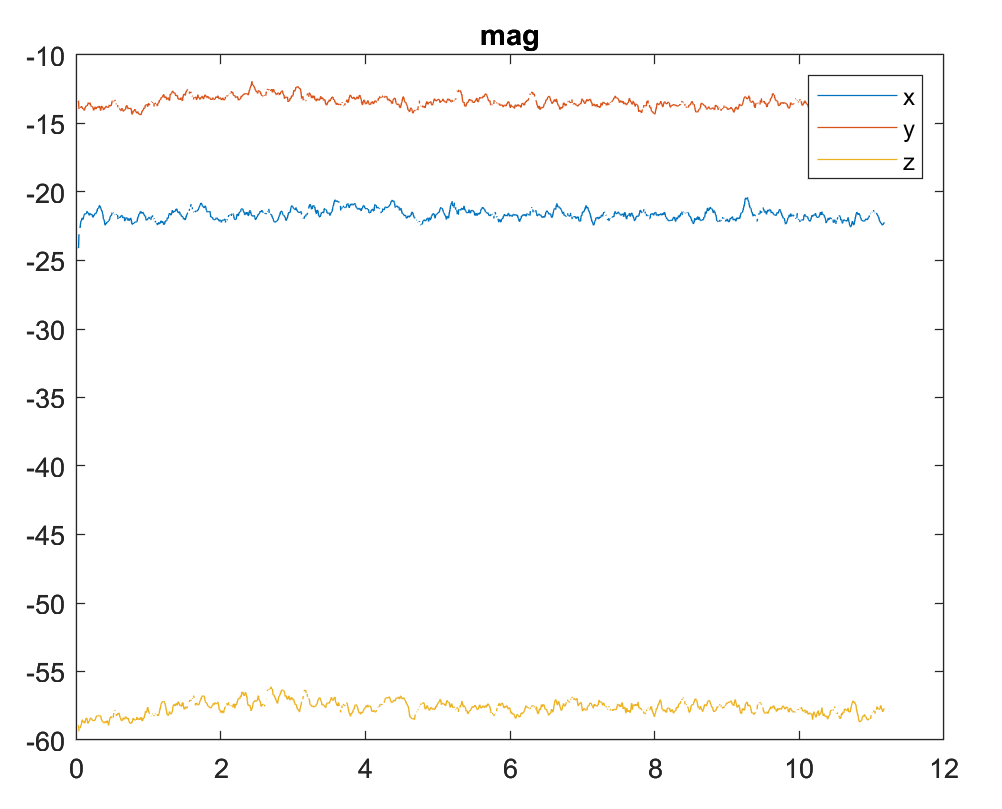
\includegraphics[width=0.7\textwidth]{images/magnetometers.png}
 \caption{Magnetometers}
 \label{mag}
\end{figure}

Through observation of the sensor plots, it is evident that when the phone is placed flat on a table, the readings from all three sensors demonstrate a consistent and stable trend without notable disturbances.


\subsection{Mean and covariance and histograms}

\begin{figure}[H]
 \centering
 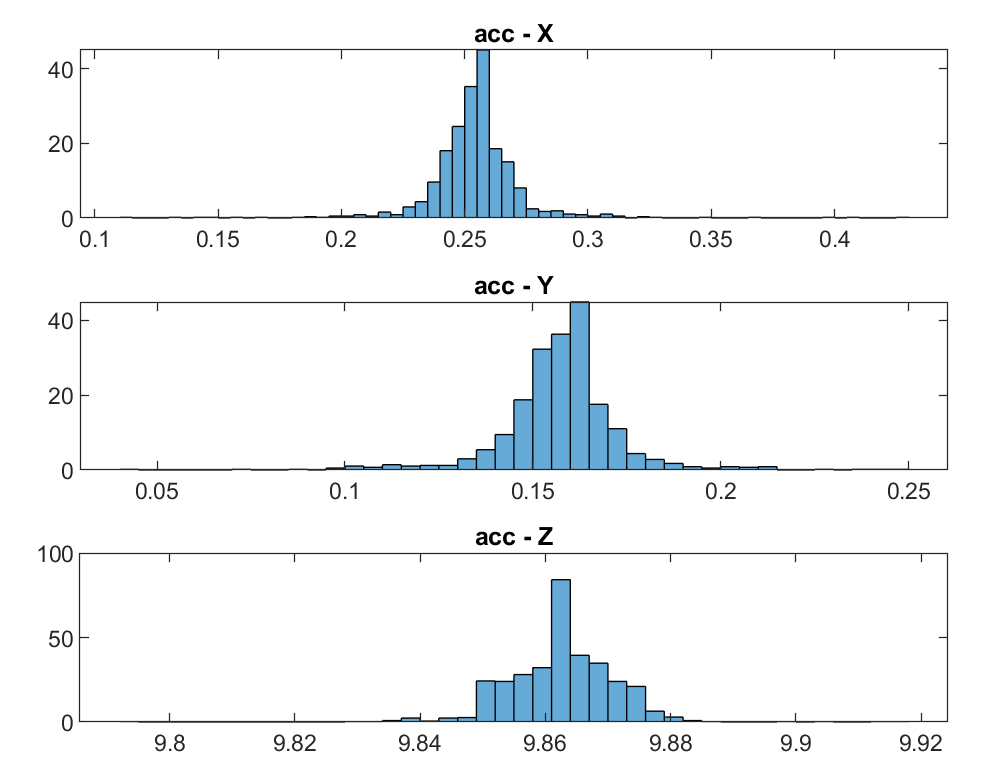
\includegraphics[width=0.7\textwidth]{images/histogramacc.png}
 \caption{Histograms for accelerometers}
 \label{hisacc}
\end{figure}

The mean of acc -X is 0.254171 , the covariance of acc -X is 0.019724  

The mean of acc -Y is 0.157052 , the covariance of acc -Y is 0.016096 

The mean of acc -Z is 9.862452 , the covariance of acc -Z is 0.008445 

\begin{figure}[H]
 \centering
 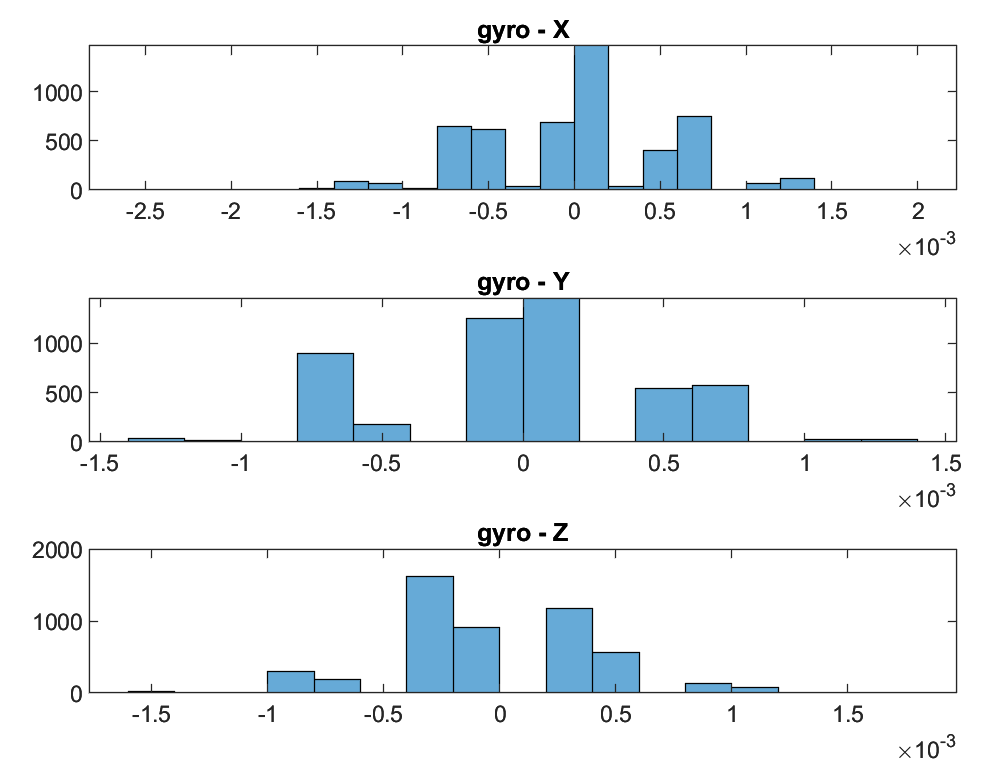
\includegraphics[width=0.7\textwidth]{images/histogramgyroscope.png}
 \caption{Histograms for gyroscope}
 \label{hisgyro}
\end{figure}


The mean of gyro -X is 0.000014 
, the covariance of gyro -X is 0.000554  

The mean of gyro -Y is -0.000031 
, the covariance of gyro -Y is 0.000449 

The mean of gyro -Z is -0.000025 
, the covariance of gyro -Z is 0.000453 

\begin{figure}[H]
 \centering
 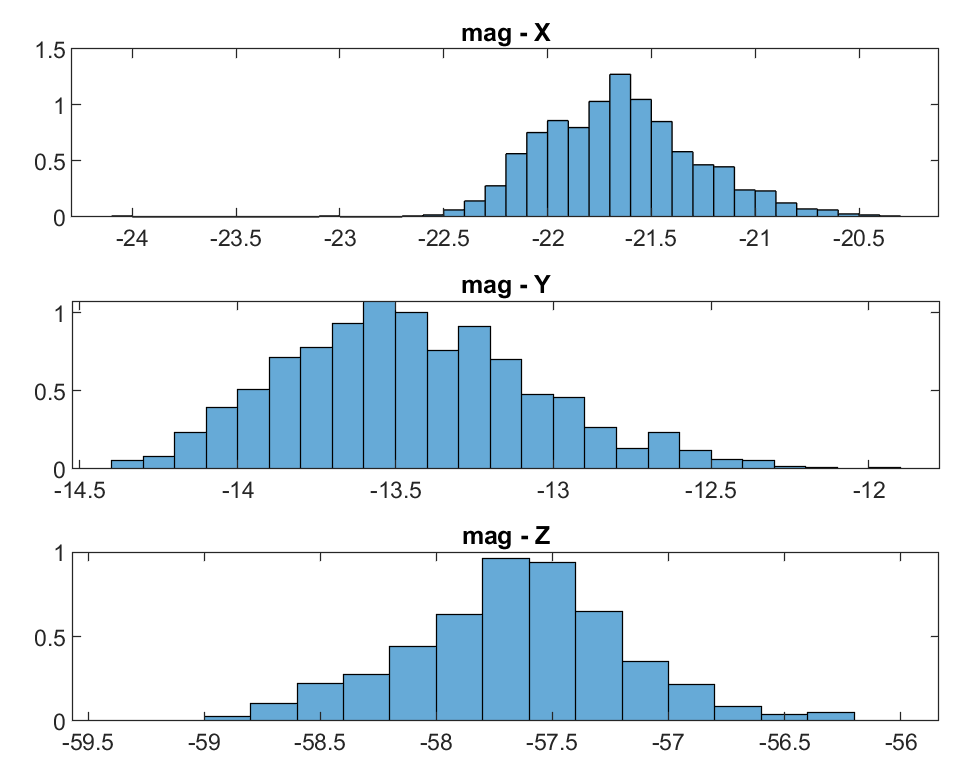
\includegraphics[width=0.7\textwidth]{images/hismagnetometer.png}
 \caption{Histograms for magnetometers}
 \label{hismag}
\end{figure}

The mean of mag -X is -21.648532 
, the covariance of mag -X is 0.377973  

The mean of mag -Y is -13.445163 
, the covariance of mag -Y is 0.401212 

The mean of mag -Z is -57.647071 
, the covariance of mag -Z is 0.477309 




The histogram of the accelerometer (acc) displays a distribution closely resembling a Gaussian shape, with a slight offset around the mean. This offset can likely be attributed to initial calibration errors during sensor measurements. Considering the protrusion of the rear camera on my phone, it is plausible that the mean offset of the accelerometer is influenced by the components of gravitational acceleration along the corresponding coordinate axes. As the phone is unlikely to be placed on a table for future measurements, this error can be mitigated. Therefore, it is reasonable to treat the accelerometer noise as Gaussian noise.

The histogram of the gyroscope (gyro) does not precisely align with a Gaussian distribution. This discrepancy may be due to the extremely small measurement errors of the gyroscope. Even if there are some offsets, the histogram shape may not exhibit a pronounced Gaussian distribution due to the minimal presence of noise. The noise in the gyroscope is exceptionally small, rendering it highly reliable. Therefore, during the subsequent tuning process, it can be assumed to have negligible measurement model noise and set to zero.

The histogram of the magnetometer (mag) exhibits a shape resembling a Gaussian distribution, albeit with an overall offset. This offset could be influenced by environmental noise in the magnetic field or biases in the magnetometer. To ensure accurate measurements, it is recommended to calibrate the magnetometer based on the current environment before each use, taking into account the specific requirements of the subsequent content.


In the subsequent experiments, I placed the mobile phone on a roll of paper to ensure that the mobile phone's XY plane was parallel to the table as much as possible. This also extended the measurement time. Therefore, new measurement values were used in the last few tasks, but they were all based on the \texttt{calculation} function.


\section{Design the EKF time update step}

\subsection{Task 3}

To derive a discretized model from the continuous time model in equation (5), we can solve the differential equation and use the relation $exp(AΔt) \approx I + AΔt$ to obtain the discretized form. Here's the derivation:


Starting with the continuous-time model:
$\dot{q}(t) = \frac{1}{2}S(\omega_{k-1}+v_{k-1})q(t), \text{ for } t \in [t_{k-1}, t_k),$

Integrating both sides of the equation from $t_{k-1}$ to $t_k$, we have:
$\int_{t_{k-1}}^{t_k} \dot{q}(t) dt = \int_{t_{k-1}}^{t_k} \frac{1}{2}S(\omega_{k-1}+v_{k-1})q(t) dt.$

Applying the integral on the left side:
$q(t_k) - q(t_{k-1}) = \frac{1}{2}S(\omega_{k-1}+v_{k-1})\int_{t_{k-1}}^{t_k} q(t) dt.$

Using the relation $exp(AΔt) ≈ I + AΔt$, where $Δt = t_k - t_{k-1}$, we can approximate the integral term:
$\int_{t_{k-1}}^{t_k} q(t) dt \approx \Delta t \cdot q(t_{k-1}).$

Substituting this approximation back into the equation:
$q(t_k) - q(t_{k-1}) = \frac{1}{2}S(\omega_{k-1}+v_{k-1})\Delta t \cdot q(t_{k-1}).$

Rearranging the equation, we get:
$q(t_k) = (I + \frac{1}{2}\Delta t \cdot S(\omega_{k-1}+v_{k-1})) \cdot q(t_{k-1}).$

Comparing this with the discretized model $q_k = F(\omega_{k-1})q_{k-1} + G(\hat{q}_{k-1})v_{k-1},$ we can identify the expressions for $F$ and $G$ as follows:

$F(\omega_{k-1}) = I + \frac{1}{2}T\cdot S(\omega_{k-1}),$

$G(\hat{q}_{k-1}) = \frac{1}{2}T \cdot S(\hat{q}_{k-1}).$

Note: These derivation above is too weird that it reached the same result but the procedure is totally different.

\emph{Note2} :OK from combine slides and the report of Linkoping university, we can reach the same result.


\subsubsection{Reason for Discretize}

In the EKF, the prediction step involves propagating the state estimate and covariance from the previous time step to the current time step. This propagation is typically done using the continuous-time dynamic model, which can be linearized around the current state estimate. However, linearizing the model can introduce errors, especially for highly nonlinear systems.

To address this issue, the discretized model derived using the approximation techniques provides an alternative approach for the prediction step in the EKF. By discretizing the continuous-time dynamic model, we can directly apply it in the discrete-time domain without the need for linearization. This allows us to capture the nonlinearities of the system more accurately, especially when the nonlinearities are significant.

\subsection{Task 4}

If there are angular velocities, update the estimate and covariance as motion model, in function \texttt{tu\_qw}.

Once $ v_k $ is missing, use the same consideration as in homework 2, skip the update for current time and keep the state and covariance value as the latest update value.

\subsection{Task 5}

In the function \texttt{Task5\_filterTemple}, I applied the \texttt{tu\_qw} and \texttt{mu\_normalizeQ} functions for the sensor \emph{gyro}.

As observed and analysed before, \emph{gyro} is accurate for the angular velocities, but it can not accually get the absolute orientation.

So when I start from the phone face to left and stand on it left edge, it takes it as the intial flat state. In the process I shake it, it always has a bias, or to say, offset with the Goolge estimate figure.

\emph{Gyro} also has a feature that I will drift according to bias. So when I start with the phone on the table, shake it for some time and place it back, repeat this procedure twice, it clearly shows a dift process in figure \ref{fig:drift-process}:


\begin{figure}[H]
    \centering
    \begin{subfigure}[H]{0.3\textwidth}
        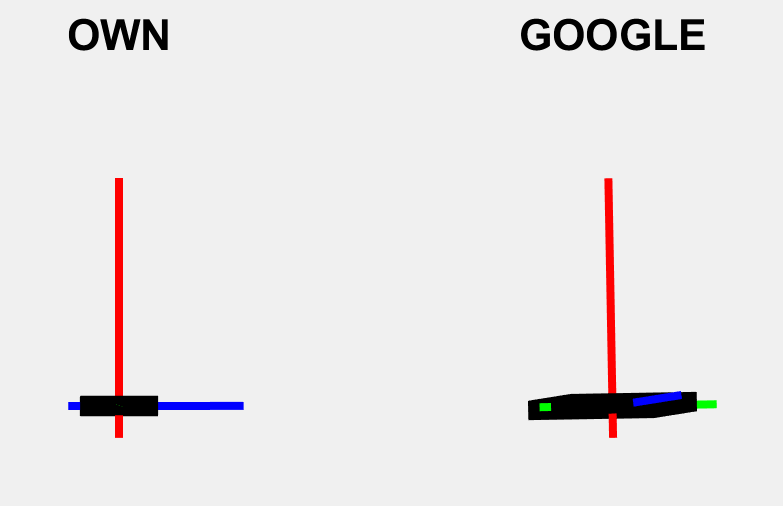
\includegraphics[width=\textwidth]{images/beginning.png}
        \caption{Begin}
        \label{fig:begin}
    \end{subfigure}
    \hfill
    \begin{subfigure}[H]{0.3\textwidth}
        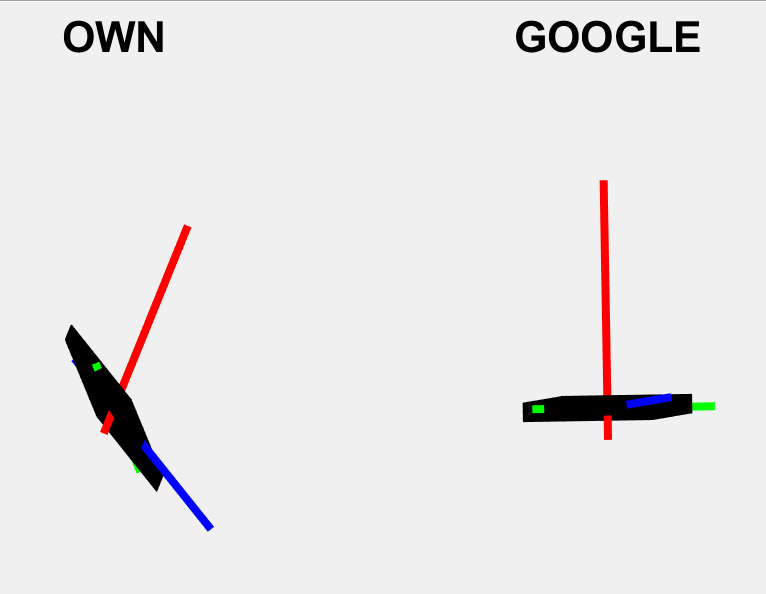
\includegraphics[width=\textwidth]{images/drift1.png}
        \caption{Firstshake}
        \label{fig:drift1}
    \end{subfigure}
    \hfill
    \begin{subfigure}[H]{0.3\textwidth}
        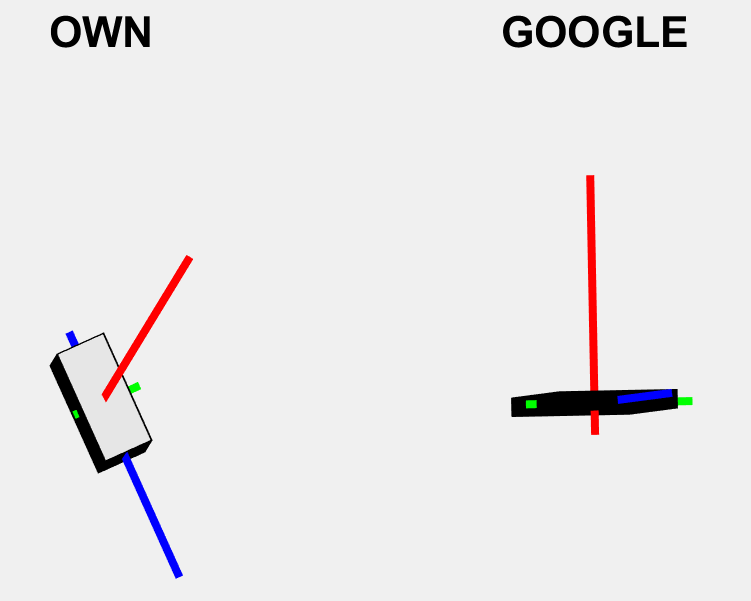
\includegraphics[width=\textwidth]{images/drift2.png}
        \caption{Secondshake}
        \label{fig:drift2}
    \end{subfigure}
    \caption{Drift Process}
    \label{fig:drift-process}
\end{figure}




\section{MMSE and MAP estimators}

\subsection{a}

\begin{figure}[H]
 \centering
 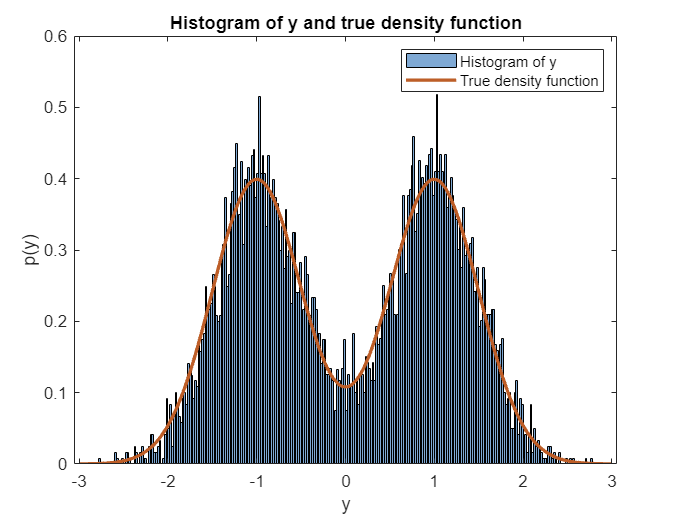
\includegraphics[width=0.7\textwidth]{images/graphfor4a.png}
 \caption{Sample 3000 times }
 \label{4a}
\end{figure}

Since $\theta$ is equally likely to be -1 or 1, the histogram of y should show two normal distributions with means -1 and 1 and equal variances $\sigma^2 = 0.25$. The overall shape of the histogram should be a bimodal distribution, with two peaks at -1 and 1 and equal weights. This bimodal distribution represents a mixture of two normal distributions, each with a different mean and the same variance.

\subsection{b}

\emph{Note: In my homework, solving b is after c. So I used the conclusions in c to prove b while.}

In this problem, we are given that $y = \theta + w$, where $w \sim N(0, 0.25)$ is a normally distributed noise term with mean 0 and variance 0.25. Therefore, the probability density function of y given theta is given by:

$$p(y | \theta) = \frac{1}{\sqrt{2\pi\sigma^2}} \exp \left(-\frac{(y - \theta)^2}{2\sigma^2}\right)$$

From c, we get:

$$p(y) = 0.5 \cdot \frac{1}{\sqrt{2 \pi \sigma^2}} \exp \left(-\frac{(y - 1)^2}{2 \sigma^2}\right) + 0.5 \cdot \frac{1}{\sqrt{2 \pi \sigma^2}} \exp \left(-\frac{(y + 1)^2}{2 \sigma^2}\right)$$

Substituting $y=0.7$ and $sigma^2$ = 0.25, we obtain:
\begin{lstlisting}
q = @(theta,y) 1/sqrt(2*pi*sigma2)*exp(-(y-theta)^2/(2*sigma2));
q(1,0.7)
ans =

    0.6664


f = @(y) 0.5*1/sqrt(2*pi*sigma2)*exp(-(y-1)^2/(2*sigma2))+0.5*1/sqrt(2*pi*sigma2)*exp(-(y+1)^2/(2*sigma2));
f(0.7)

ans =

    0.3345
\end{lstlisting}

so:

$p(\theta=1 | y=0.7) = \frac{p(y=0.7 | \theta=1) p(\theta=1)}{p(y=0.7)} = \frac{0.6664\times0.5}{0.3345}=0.9961$

$$p(\theta=-1 | y=0.7) = 0.0039$$

So I guess $ \theta $ =1.

\subsection{c}

To prove that $p(y)$ is a mixture of two normal distributions with means $-1$ and $1$ and the same variance $\sigma^2$, we can use the law of total probability.

In this problem, we can partition the sample space of $y$ into two mutually exclusive events: $y = \theta + w$ where $\theta = 1$ and $\theta = -1$, where $w \sim \mathcal{N}(0, \sigma^2)$ is a normally distributed noise term with mean $0$ and variance $\sigma^2$. 

Using the law of total probability, we can express $p(y)$ as a mixture of the two normal distributions as follows:

$$p(y) = p(y | \theta = 1) p(\theta = 1) + p(y | \theta = -1) p(\theta = -1)$$

where $p(y | \theta = 1)$ is the probability density function of the normal distribution with mean $1$ and variance $\sigma^2$, and $p(y | \theta = -1)$ is the probability density function of the normal distribution with mean $-1$ and variance $\sigma^2$.

Substituting the expressions for the two probability density functions, we obtain:

$$p(y) = 0.5 \cdot \frac{1}{\sqrt{2 \pi \sigma^2}} \exp \left(-\frac{(y - 1)^2}{2 \sigma^2}\right) + 0.5 \cdot \frac{1}{\sqrt{2 \pi \sigma^2}} \exp \left(-\frac{(y + 1)^2}{2 \sigma^2}\right)$$

Therefore, $p(y)$ is a mixture of two normal distributions with means $-1$ and $1$ and the same variance $\sigma^2$.

\subsection{d}

The Bayesian rule says:
\begin{equation}
    \begin{aligned}
        p(\theta|y)= \frac{p(y|\theta)}{p(y)}\nonumber
    \end{aligned}
\end{equation}

Already known $ p(y) $ in question c and $ p(y|\theta) $ in question b, so:

\begin{equation}
    \begin{aligned}
        p(\theta|y)&=\begin{cases}\frac{\frac{1}{2}\frac{1}{\sqrt{2\pi}\sigma}\exp\{-\frac{1}{2\sigma^2}(y-1)^2\}}{\frac{1}{2}\frac{1}{\sqrt{2\pi}\sigma}\exp\{-\frac{1}{2\sigma^2}(y-1)^2\}+\frac{1}{2}\frac{1}{\sqrt{2\pi}\sigma}\exp\{-\frac{1}{2\sigma^2}(y+1)^2\}}& \text{if } \theta =1\\ \frac{\frac{1}{2}\frac{1}{\sqrt{2\pi}\sigma}\exp\{-\frac{1}{2\sigma^2}(y+1)^2\}}{\frac{1}{\sqrt{2\pi}\sigma}\exp\{-\frac{1}{2\sigma^2}(y-1)^2\}+\frac{1}{2}\frac{1}{\sqrt{2\pi}\sigma}\exp\{-\frac{1}{2\sigma^2}(y+1)^2\}}&\text{if } \theta=-1\end{cases}\\
        &=\begin{cases}\frac{\exp\{\frac{y}{\sigma^2}\}}{\exp\{\frac{y}{\sigma^2}\}+\exp\{-\frac{y}{\sigma^2}\}}&\text{if } \theta =1\\ \frac{\exp\{\frac{-y}{\sigma^2}\}}{\exp\{\frac{y}{\sigma^2}\}+\exp\{-\frac{y}{\sigma^2}\}}&\text{if } \theta =-1\end{cases}\\
        &\text{where  }  \sigma^2=0.25\nonumber
    \end{aligned} 
\end{equation}

\subsection{e}

\begin{equation}
    \begin{aligned}
        \:\hat{\theta}_{M M S E}&=\sum_{\theta}\theta\operatorname*{Pr}\{\theta|y\}.\:\\
        &=p(\theta=1|y)-p(\theta=-1|y)\\
        &=\dfrac{\exp\frac{y}{\sigma^2}-\exp-\frac{y}{\sigma^2}}{\exp\frac{y}{\sigma^2}+\exp-\frac{y}{\sigma^2}}\\
        &=\:\:\frac{2\sinh\left(\frac{y}{\sigma^2}\right)}{2\cosh\left(\frac{y}{\sigma^2}\right)}=\tanh\left(\frac{y}{\sigma^2}\right)=tanh(4y)\nonumber
    \end{aligned}
\end{equation}

\subsection{f}

\begin{equation}
    \begin{aligned}
        \hat{\theta}_{MAP}&=\arg\max\limits_{\theta=\pm1}\pi_y(\theta)\nonumber\\
        &=\begin{cases}1& \text{if } \frac{\exp\frac{y}{\sigma^2}}{\exp\frac{y}{\sigma^2}+\exp-\frac{y}{\sigma^2}}\geq\frac{\exp-\frac{y}{\sigma^2}}{\exp\frac{y}{\sigma^2}+\exp-\frac{y}{\sigma^2}}\\-1& \text{if } \frac{{\exp}\frac{y}{\sigma^2}}{\exp\frac{y}{\sigma^2}+\exp-\frac{y}{\sigma^2}}<\frac{{\exp}-\frac{y}{\sigma^2}}{\exp\frac{y}{\sigma^2}+\exp-\frac{y}{\sigma^2}}\end{cases}\\
        &=\begin{cases}1& \text{if } y\geq 0\\-1 & \text{if } y \leq 0 \end{cases}
    \end{aligned}
\end{equation}

\subsection{g}
\subsubsection{1}

In 4b), we made the guess that $\theta$ is 1. Meanwhile, for the specific value of $y=0.7$, both the MMSE estimator and the MAP estimator would predict that $\theta$ is 1. In this case, our guess in 4b coincides with both the MMSE and MAP estimators.

\subsubsection{2}

In this problem, the MMSE and MAP estimators for $\theta$ are different. The MMSE estimator is given by $\hat{\theta}_{MMSE} = \tanh(4y)$, while the MAP estimator is given by $\hat{\theta}_{MAP} = \operatorname{sgn}(y)$.

The MMSE estimator minimizes the expected squared error between the estimated value of $\theta$ and the true value, while the MAP estimator maximizes the posterior probability of $\theta$ given the observation $y$. In this case, the MMSE estimator and the MAP estimator make different decisions when $y$ is close to 0.

If $y$ is positive, both the MMSE and MAP estimators predict that $\theta$ is 1. If $y$ is negative, the MMSE estimator predicts that $\theta$ is -1, while the MAP estimator predicts that $\theta$ is 1. This is because the MMSE estimator takes into account the entire posterior distribution of $\theta$, while the MAP estimator only considers the most probable value of $\theta$.


%%%%%%%%%%%%%%%%%%%%%%%%%%%%%%%%%%%%%%%%%%%%%%%%%%%%%%%%%%%%%
\end{document}
